\chapter{Results and Discussion}
\label{ch:results}

\section{Primary Performance Metrics}

The model was tested on a separate test set of 1,132 images and had an overall accuracy of 96.6\%. For the class generated by AI, the precision achieved 98.9\%, recall 95.3\% and an F1-Score of 97.0\%, which reflects good balance in minimising false-positives and negative. The AUC-ROC score is calculated for the plots of 0.992 further demonstrates near perfect class-separability at every classification threshold. Inference latency was measured to be 142.4 ms on CPU using a Hugging Face Spaces environment which is still decent enough when it comes to real-world deployment without GPU resources.

\begin{table}[htbp]
    \centering
    \caption{Primary performance metrics on the held-out test set.}
    \label{tab:metrics}
    \begin{tabular}{lc}
        \toprule
        \textbf{Metric} & \textbf{Value} \\
        \midrule
        Accuracy                          & 96.6\% \\
        Precision (AI class)              & 98.9\% \\
        Recall (AI class)                 & 95.3\% \\
        F1-Score (AI class)               & 97.0\% \\
        AUC-ROC                           & 0.992 \\
        Inference Latency (CPU, HF Spaces) & 142.4 ms \\
        \bottomrule
    \end{tabular}
\end{table}

\section{Confusion Matrix Analysis}

As shown in Figure 5.1, out of 472 images created by humans, 465 images were classified correctly and only 7 images were mistakenly flagged as AI-generated (false positive rate is only 1.5\%). Of the 660 AI-generated images, 629 were correctly identified while 31 of those images were misclassified as human because of the likely fact that the AI images closely mimicked human artistic styles. The significantly lower number of false positives than false negatives is symptomatic of the model's tendency to be conservative in labelling human content as AI generated, which is a desirable property in sensitive deployment contexts, in which misclassification of content genuinely produced by human writers has more severe consequences.

\begin{figure}[H]
    \centering
    % NOTE: Place the confusion matrix image in img/confusion_matrix.png
    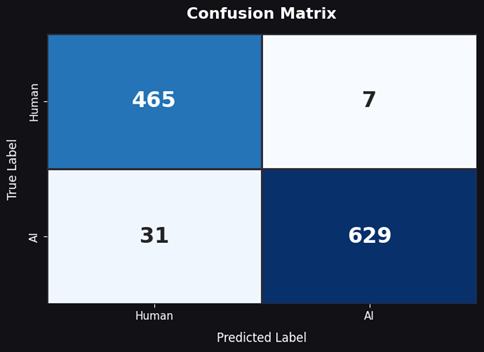
\includegraphics[width=0.75\textwidth]{img/confusion_matrix}
    \caption{Confusion matrix on the held-out test set of 1,132 images.}
    \label{fig:confusion}
\end{figure}

\section{ROC Curve and AUC Analysis}

\begin{figure}[htbp]
    \centering
    % NOTE: Place the ROC curve image in img/roc_curve.png
    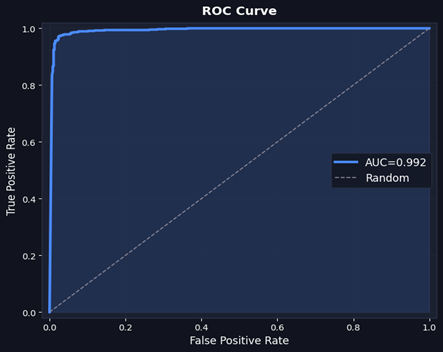
\includegraphics[width=0.7\textwidth]{img/roc_curve}
    \caption{Receiver Operating Characteristic (ROC) curve for the proposed hybrid model.}
    \label{fig:roc}
\end{figure}

Receiver Operating Characteristic (ROC curve) is the probability curve for all possible TPR and FPR classification thresholds. An AUC-ROC of 0.992 means that the classifier can discriminate, or in laymen terms, there is a 99.2\% of probability that if you randomly draw an AI “fake” image and a random actual image the fake image would get the higher probability score”. And from ROC curve - the model has its True Positive Rate (TPR) greater than 99\% while still maintaining a False Positive Rate (FPR) lesser than 3\%. “This clearly shows that a precision-recall trade off can be improved by lowering the classification threshold, without sacrificing recall”.

\section{Comparison with Commercial Detection Tools}

A qualitative comparative study was carried out using a set of hard-negative AI-generated images. These images are of high quality, with no obvious visual artifacts, making them challenging to detection models. The same set of images was passed through two detection tools, Undetectable AI and AI or Not, along with the proposed model, and the results obtained are shown in Table~\ref{tab:comparison}.

\begin{table}[htbp]
    \centering
    \caption{Comparative analysis on a representative hard-negative AI-generated image.}
    \label{tab:comparison}
    \begin{tabular}{p{4.5cm} p{5.5cm} p{2.5cm}}
        \toprule
        \textbf{Detector} & \textbf{Verdict} & \textbf{Latency} \\
        \midrule
        Proposed Model (Ours)        & AI-Generated (100\% confidence) & 142.4 ms \\
        AI or Not (Commercial)       & Likely REAL                     & 920 ms \\
        Undetectable AI (Commercial) & 98\% REAL                       & 5,230 ms \\
        \bottomrule
    \end{tabular}
\end{table}

\begin{figure}[htbp]
    \centering
    % NOTE: Place the commercial comparison screenshots in img/ folder
    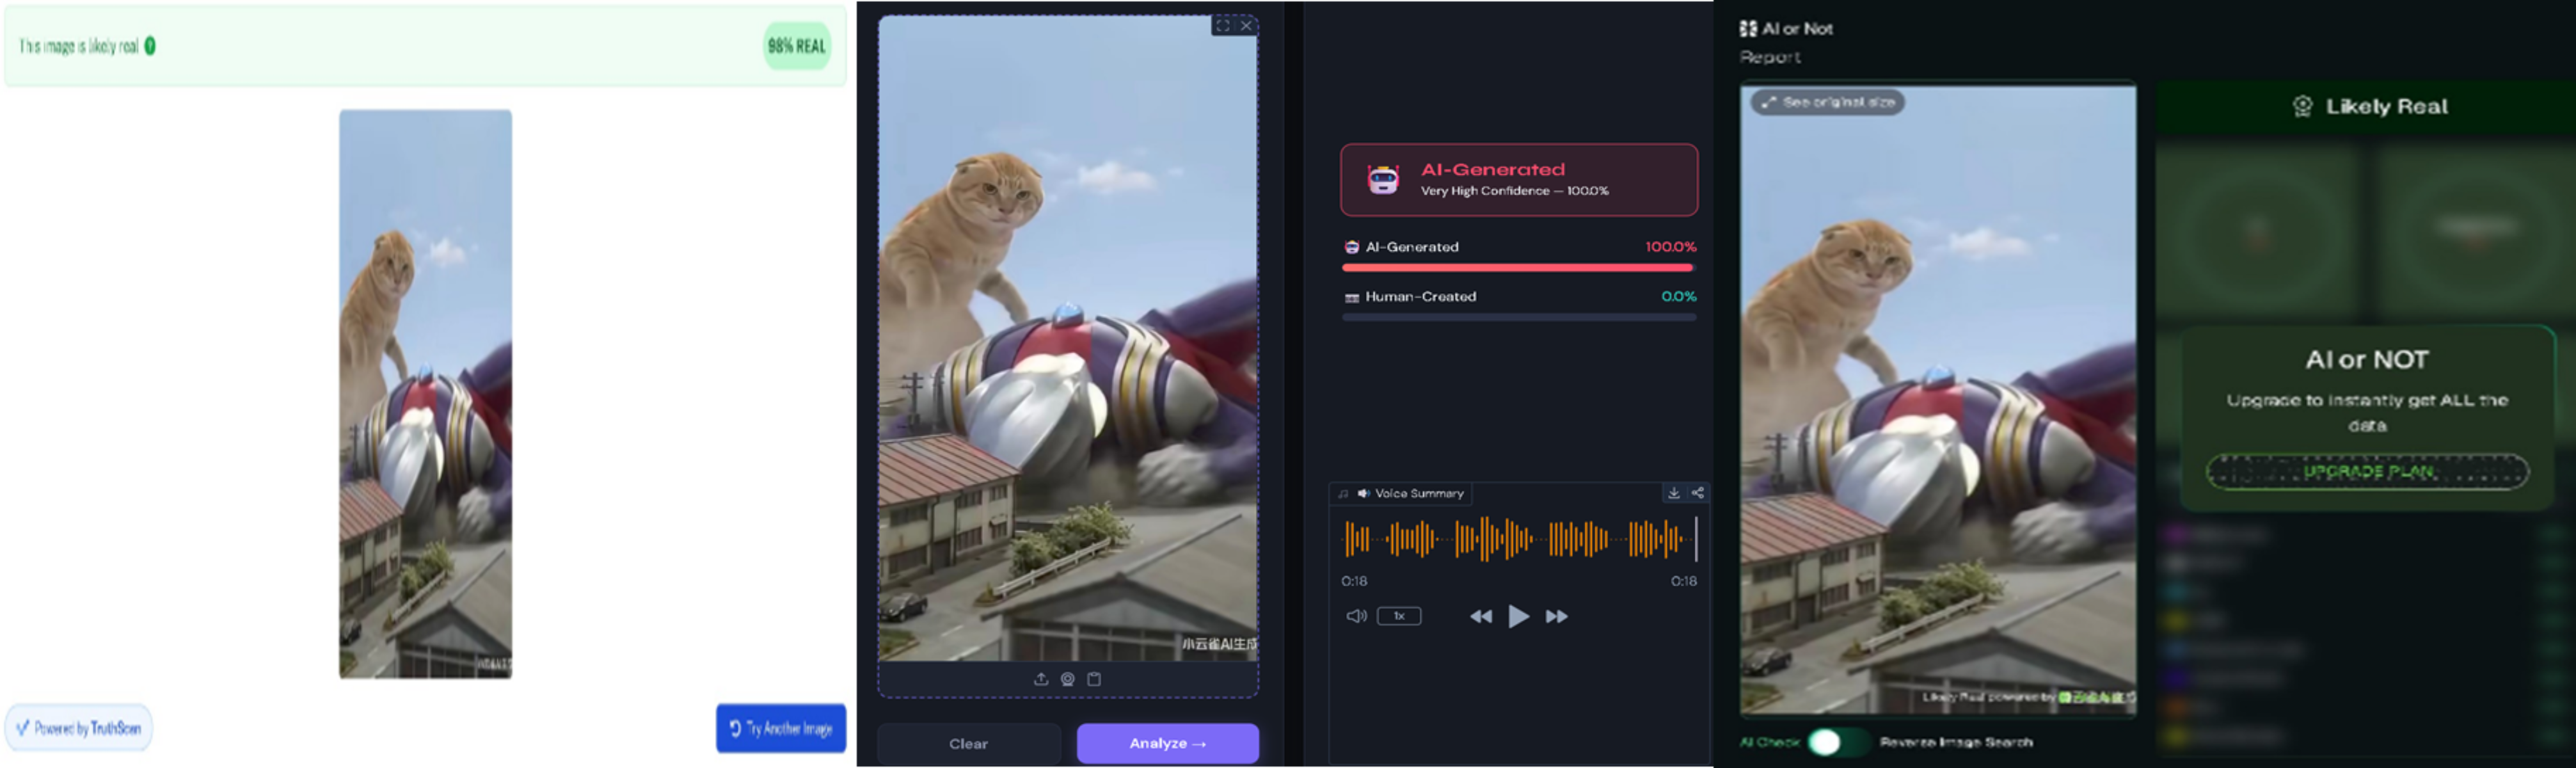
\includegraphics[width=0.65\textwidth]{img/commercial_comparison}
    \caption{Hard-negative test case: comparison of detection results across our model and commercial tools.}
    \label{fig:commercial}
\end{figure}

The results demonstrate two important advantages of the proposed architecture. First, the proposed model correctly identifies the hard-negative image as AI-generated with 100\% confidence, while both commercial tools misclassify it as real. This superior accuracy on hard negatives is attributable to the combination of the SigLIP 2 backbone's rich visual representations with the traditional forensic features, which collectively detect signatures that are not visually apparent but are statistically distinguishable. Second, the proposed model achieves this result in 142.4 milliseconds---$6.5\times$ faster than AI or Not (920 ms) and $36.7\times$ faster than Undetectable AI (5,230 ms). At 142.4 ms per image, the proposed model can process approximately 7 images per second, making it viable for integration into real-time content moderation pipelines, whereas the commercial tools would process fewer than 1 image per second on the same hardware.

\section{Discussion and Interpretation}

The results demonstrate that the proposed hybrid architecture successfully achieves the primary research objective: a single-pass AI image detector that matches the accuracy of heavy ensemble systems while operating at inference speeds suitable for real-time deployment. The 0.992 AUC-ROC places the model firmly within the range of top-performing ensemble systems reported in prior benchmark studies \cite{perotti2025nodedetector, li2025aigibench}, while the 142.4 ms inference latency is a significant improvement over commercial platforms and approaches the real-time threshold.

The main conclusion supported by these findings is that traditional forensic features and deep visual features are complementary, rather than redundant, features. The SigLIP 2 backbone, trained on 10 billion image-text pairs \cite{tschannen2025siglip2}, has learned features that are sensitive to high-level visual and semantic properties that distinguish AI-generated images from real images. The traditional features, obtained from physical models of camera image formation, capture low-level statistical properties in the frequency, noise, and texture domains, which are largely inaccessible to attention-based models operating at the feature map level. The use of the SE-style attention mechanism in the classification head learns how to dynamically weight the relative importance of the two signal streams, effectively performing a learned feature selection depending on the properties of each image artifact.

The improved performance on hard-negative images, especially those images classified correctly when commercial tools fail, provides perhaps the most compelling evidence supporting this hybrid approach. By definition, hard-negative images do not contain visually obvious AI artifacts, and detection relies on reasoning about statistical properties, which are physically meaningful and perceptually subtle. The traditional features, especially the Bayer noise pattern, which detects the absence of camera demosaicing fingerprints, and the DCT Benford deviation, which detects violations of natural frequency statistics, provide a discriminative signal that is absent in AI-generated images.
